% Options for packages loaded elsewhere
\PassOptionsToPackage{unicode}{hyperref}
\PassOptionsToPackage{hyphens}{url}
\PassOptionsToPackage{dvipsnames,svgnames,x11names}{xcolor}
%
\documentclass[
  letterpaper,
  DIV=11,
  numbers=noendperiod]{scrartcl}

\usepackage{amsmath,amssymb}
\usepackage{iftex}
\ifPDFTeX
  \usepackage[T1]{fontenc}
  \usepackage[utf8]{inputenc}
  \usepackage{textcomp} % provide euro and other symbols
\else % if luatex or xetex
  \usepackage{unicode-math}
  \defaultfontfeatures{Scale=MatchLowercase}
  \defaultfontfeatures[\rmfamily]{Ligatures=TeX,Scale=1}
\fi
\usepackage{lmodern}
\ifPDFTeX\else  
    % xetex/luatex font selection
\fi
% Use upquote if available, for straight quotes in verbatim environments
\IfFileExists{upquote.sty}{\usepackage{upquote}}{}
\IfFileExists{microtype.sty}{% use microtype if available
  \usepackage[]{microtype}
  \UseMicrotypeSet[protrusion]{basicmath} % disable protrusion for tt fonts
}{}
\makeatletter
\@ifundefined{KOMAClassName}{% if non-KOMA class
  \IfFileExists{parskip.sty}{%
    \usepackage{parskip}
  }{% else
    \setlength{\parindent}{0pt}
    \setlength{\parskip}{6pt plus 2pt minus 1pt}}
}{% if KOMA class
  \KOMAoptions{parskip=half}}
\makeatother
\usepackage{xcolor}
\setlength{\emergencystretch}{3em} % prevent overfull lines
\setcounter{secnumdepth}{5}
% Make \paragraph and \subparagraph free-standing
\ifx\paragraph\undefined\else
  \let\oldparagraph\paragraph
  \renewcommand{\paragraph}[1]{\oldparagraph{#1}\mbox{}}
\fi
\ifx\subparagraph\undefined\else
  \let\oldsubparagraph\subparagraph
  \renewcommand{\subparagraph}[1]{\oldsubparagraph{#1}\mbox{}}
\fi

\usepackage{color}
\usepackage{fancyvrb}
\newcommand{\VerbBar}{|}
\newcommand{\VERB}{\Verb[commandchars=\\\{\}]}
\DefineVerbatimEnvironment{Highlighting}{Verbatim}{commandchars=\\\{\}}
% Add ',fontsize=\small' for more characters per line
\usepackage{framed}
\definecolor{shadecolor}{RGB}{241,243,245}
\newenvironment{Shaded}{\begin{snugshade}}{\end{snugshade}}
\newcommand{\AlertTok}[1]{\textcolor[rgb]{0.68,0.00,0.00}{#1}}
\newcommand{\AnnotationTok}[1]{\textcolor[rgb]{0.37,0.37,0.37}{#1}}
\newcommand{\AttributeTok}[1]{\textcolor[rgb]{0.40,0.45,0.13}{#1}}
\newcommand{\BaseNTok}[1]{\textcolor[rgb]{0.68,0.00,0.00}{#1}}
\newcommand{\BuiltInTok}[1]{\textcolor[rgb]{0.00,0.23,0.31}{#1}}
\newcommand{\CharTok}[1]{\textcolor[rgb]{0.13,0.47,0.30}{#1}}
\newcommand{\CommentTok}[1]{\textcolor[rgb]{0.37,0.37,0.37}{#1}}
\newcommand{\CommentVarTok}[1]{\textcolor[rgb]{0.37,0.37,0.37}{\textit{#1}}}
\newcommand{\ConstantTok}[1]{\textcolor[rgb]{0.56,0.35,0.01}{#1}}
\newcommand{\ControlFlowTok}[1]{\textcolor[rgb]{0.00,0.23,0.31}{#1}}
\newcommand{\DataTypeTok}[1]{\textcolor[rgb]{0.68,0.00,0.00}{#1}}
\newcommand{\DecValTok}[1]{\textcolor[rgb]{0.68,0.00,0.00}{#1}}
\newcommand{\DocumentationTok}[1]{\textcolor[rgb]{0.37,0.37,0.37}{\textit{#1}}}
\newcommand{\ErrorTok}[1]{\textcolor[rgb]{0.68,0.00,0.00}{#1}}
\newcommand{\ExtensionTok}[1]{\textcolor[rgb]{0.00,0.23,0.31}{#1}}
\newcommand{\FloatTok}[1]{\textcolor[rgb]{0.68,0.00,0.00}{#1}}
\newcommand{\FunctionTok}[1]{\textcolor[rgb]{0.28,0.35,0.67}{#1}}
\newcommand{\ImportTok}[1]{\textcolor[rgb]{0.00,0.46,0.62}{#1}}
\newcommand{\InformationTok}[1]{\textcolor[rgb]{0.37,0.37,0.37}{#1}}
\newcommand{\KeywordTok}[1]{\textcolor[rgb]{0.00,0.23,0.31}{#1}}
\newcommand{\NormalTok}[1]{\textcolor[rgb]{0.00,0.23,0.31}{#1}}
\newcommand{\OperatorTok}[1]{\textcolor[rgb]{0.37,0.37,0.37}{#1}}
\newcommand{\OtherTok}[1]{\textcolor[rgb]{0.00,0.23,0.31}{#1}}
\newcommand{\PreprocessorTok}[1]{\textcolor[rgb]{0.68,0.00,0.00}{#1}}
\newcommand{\RegionMarkerTok}[1]{\textcolor[rgb]{0.00,0.23,0.31}{#1}}
\newcommand{\SpecialCharTok}[1]{\textcolor[rgb]{0.37,0.37,0.37}{#1}}
\newcommand{\SpecialStringTok}[1]{\textcolor[rgb]{0.13,0.47,0.30}{#1}}
\newcommand{\StringTok}[1]{\textcolor[rgb]{0.13,0.47,0.30}{#1}}
\newcommand{\VariableTok}[1]{\textcolor[rgb]{0.07,0.07,0.07}{#1}}
\newcommand{\VerbatimStringTok}[1]{\textcolor[rgb]{0.13,0.47,0.30}{#1}}
\newcommand{\WarningTok}[1]{\textcolor[rgb]{0.37,0.37,0.37}{\textit{#1}}}

\providecommand{\tightlist}{%
  \setlength{\itemsep}{0pt}\setlength{\parskip}{0pt}}\usepackage{longtable,booktabs,array}
\usepackage{calc} % for calculating minipage widths
% Correct order of tables after \paragraph or \subparagraph
\usepackage{etoolbox}
\makeatletter
\patchcmd\longtable{\par}{\if@noskipsec\mbox{}\fi\par}{}{}
\makeatother
% Allow footnotes in longtable head/foot
\IfFileExists{footnotehyper.sty}{\usepackage{footnotehyper}}{\usepackage{footnote}}
\makesavenoteenv{longtable}
\usepackage{graphicx}
\makeatletter
\def\maxwidth{\ifdim\Gin@nat@width>\linewidth\linewidth\else\Gin@nat@width\fi}
\def\maxheight{\ifdim\Gin@nat@height>\textheight\textheight\else\Gin@nat@height\fi}
\makeatother
% Scale images if necessary, so that they will not overflow the page
% margins by default, and it is still possible to overwrite the defaults
% using explicit options in \includegraphics[width, height, ...]{}
\setkeys{Gin}{width=\maxwidth,height=\maxheight,keepaspectratio}
% Set default figure placement to htbp
\makeatletter
\def\fps@figure{htbp}
\makeatother

\KOMAoption{captions}{tableheading}
\makeatletter
\makeatother
\makeatletter
\makeatother
\makeatletter
\@ifpackageloaded{caption}{}{\usepackage{caption}}
\AtBeginDocument{%
\ifdefined\contentsname
  \renewcommand*\contentsname{Table of contents}
\else
  \newcommand\contentsname{Table of contents}
\fi
\ifdefined\listfigurename
  \renewcommand*\listfigurename{List of Figures}
\else
  \newcommand\listfigurename{List of Figures}
\fi
\ifdefined\listtablename
  \renewcommand*\listtablename{List of Tables}
\else
  \newcommand\listtablename{List of Tables}
\fi
\ifdefined\figurename
  \renewcommand*\figurename{Figure}
\else
  \newcommand\figurename{Figure}
\fi
\ifdefined\tablename
  \renewcommand*\tablename{Table}
\else
  \newcommand\tablename{Table}
\fi
}
\@ifpackageloaded{float}{}{\usepackage{float}}
\floatstyle{ruled}
\@ifundefined{c@chapter}{\newfloat{codelisting}{h}{lop}}{\newfloat{codelisting}{h}{lop}[chapter]}
\floatname{codelisting}{Listing}
\newcommand*\listoflistings{\listof{codelisting}{List of Listings}}
\makeatother
\makeatletter
\@ifpackageloaded{caption}{}{\usepackage{caption}}
\@ifpackageloaded{subcaption}{}{\usepackage{subcaption}}
\makeatother
\makeatletter
\@ifpackageloaded{tcolorbox}{}{\usepackage[skins,breakable]{tcolorbox}}
\makeatother
\makeatletter
\@ifundefined{shadecolor}{\definecolor{shadecolor}{rgb}{.97, .97, .97}}
\makeatother
\makeatletter
\makeatother
\makeatletter
\makeatother
\ifLuaTeX
  \usepackage{selnolig}  % disable illegal ligatures
\fi
\IfFileExists{bookmark.sty}{\usepackage{bookmark}}{\usepackage{hyperref}}
\IfFileExists{xurl.sty}{\usepackage{xurl}}{} % add URL line breaks if available
\urlstyle{same} % disable monospaced font for URLs
\hypersetup{
  pdftitle={Working space set-up},
  pdfauthor={Johan Sáenz},
  colorlinks=true,
  linkcolor={blue},
  filecolor={Maroon},
  citecolor={Blue},
  urlcolor={Blue},
  pdfcreator={LaTeX via pandoc}}

\title{Working space set-up}
\author{Johan Sáenz}
\date{2023-05-04}

\begin{document}
\maketitle
\ifdefined\Shaded\renewenvironment{Shaded}{\begin{tcolorbox}[borderline west={3pt}{0pt}{shadecolor}, frame hidden, interior hidden, enhanced, breakable, boxrule=0pt, sharp corners]}{\end{tcolorbox}}\fi

\renewcommand*\contentsname{Table of contents}
{
\hypersetup{linkcolor=}
\setcounter{tocdepth}{3}
\tableofcontents
}
\hypertarget{working-space-set-up}{%
\section{\texorpdfstring{\textbf{Working space
set-up}}{Working space set-up}}\label{working-space-set-up}}

The most important thing to do before starting a new project is to set
up the working space. In this blog I will describe the steps that I
follow and work for me but it is not the only way. So if you find new
ways to set-up your working space feel free to do it.

\hypertarget{folder-structure}{%
\section{Folder structure}\label{folder-structure}}

\begin{enumerate}
\def\labelenumi{\arabic{enumi}.}
\tightlist
\item
  First of all, you should create a main folder with the name of the
  project and inside, you should create three sub folders call:
  \textbf{rawdata}, \textbf{code} and \textbf{figures}. The names of the
  folders indicate the type of file that would be stored in each of
  them. Sometimes I also create a folder call \textbf{processed\_data},
  when I want to save intermediate files. The file in the raw data must
  not be modified during the analysis.
\end{enumerate}

\begin{figure}[H]

{\centering 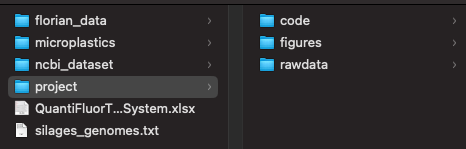
\includegraphics[width=6.25in,height=\textheight]{folders.png}

}

\end{figure}

\begin{enumerate}
\def\labelenumi{\arabic{enumi}.}
\setcounter{enumi}{1}
\tightlist
\item
  Next, You should move the raw data to the respective folder.
\item
  After, You should create a new R script and then Save as\ldots{}
  inside the \textbf{code} folder. I always give meaningful names to my
  files. Those names are based on the main goal of the script. For
  example if it is to create a bar plot, I name the file barplot.R
\end{enumerate}

\begin{figure}[H]

{\centering 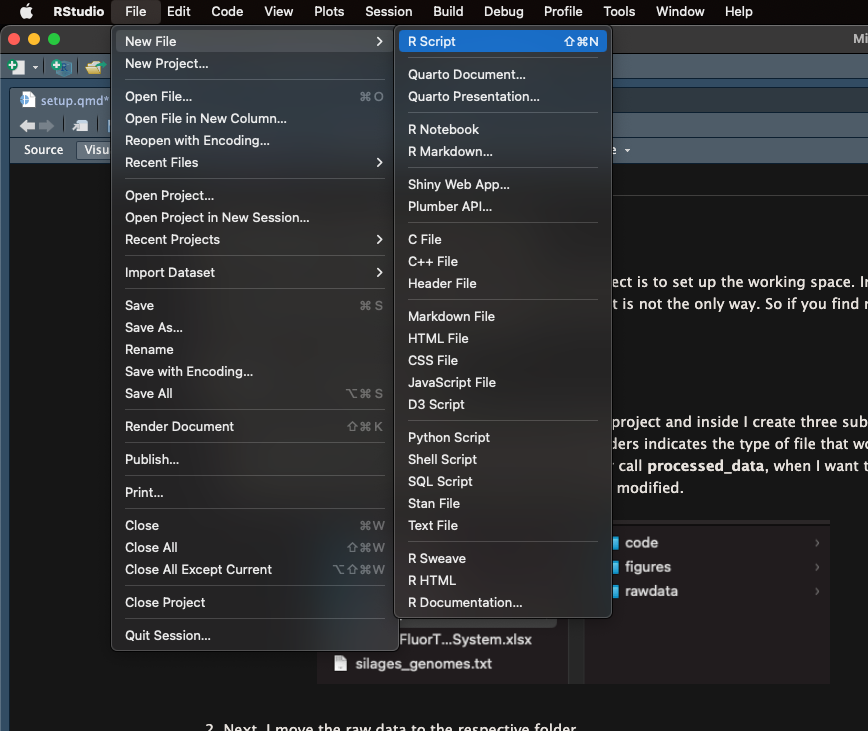
\includegraphics[width=6.25in,height=\textheight]{newfile.png}

}

\end{figure}

\hypertarget{working-directory}{%
\section{Working directory}\label{working-directory}}

\begin{enumerate}
\def\labelenumi{\arabic{enumi}.}
\setcounter{enumi}{3}
\item
  Following, You should open the new R script and use the symbol \# to
  add some comments to the file. The \# indicates that the line would
  not be run by R. The \# is quite useful as you can add different
  comments to help you and other people to understand your code.

\begin{Shaded}
\begin{Highlighting}[]
\CommentTok{\# Author: Johan S. Sáenz}
\CommentTok{\# Email: johan.saenzmedina@uni{-}hohenheim.de}
\CommentTok{\# info: script to create a barplot}
\end{Highlighting}
\end{Shaded}
\item
  Then, you should select the working directory in the Session menu. You
  should select your project folder. You will notice that in the console
  the following code was printed:
  \textbf{\texttt{setwd("/Users/sebastiansaenz/Documents/github/MicroTutorials/project")}}.
  Copy the code and paste it in your script. Add a comment indicating
  that the following line is used to set up your working directory. The
  project folder would now be consider the root directory.
\end{enumerate}

\begin{figure}[H]

{\centering 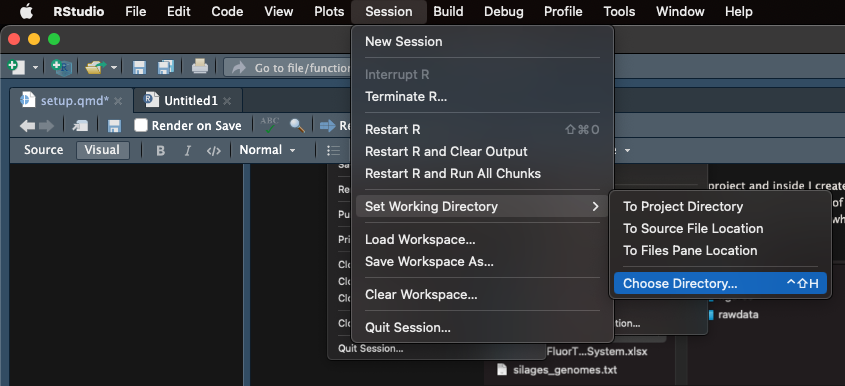
\includegraphics[width=6.25in,height=\textheight]{wd.png}

}

\end{figure}

\begin{Shaded}
\begin{Highlighting}[]
\CommentTok{\# Author: Johan S. Sáenz}
\CommentTok{\# Email: johan.saenzmedina@uni{-}hohenheim.de}
\CommentTok{\# info: script to create a barplot}

\CommentTok{\# Setting working directory}
\FunctionTok{setwd}\NormalTok{(}\StringTok{"/Users/sebastiansaenz/Documents/github/MicroTutorials/project"}\NormalTok{)}
\end{Highlighting}
\end{Shaded}

\hypertarget{installing-and-loading-libraries}{%
\section{Installing and loading
libraries}\label{installing-and-loading-libraries}}

\begin{enumerate}
\def\labelenumi{\arabic{enumi}.}
\setcounter{enumi}{5}
\tightlist
\item
  R has several pre-build functions but other packages created by the
  community can be use as long as they are install and load. Now you can
  use the function \textbf{\texttt{install.packages()}} to install the
  packages that we would need for our analysis. This function should be
  use only once, because after the installation, the package will be
  available to be load even after closing the software. On the other
  hand, the function \textbf{\texttt{library()}} must be use every time
  a new R session is initiate. After installation you can comment out
  the \textbf{\texttt{\#install.packages("tidyverse")}.} The longer you
  work in R, more new packages you will add to your collection.
\end{enumerate}

\begin{Shaded}
\begin{Highlighting}[]
\CommentTok{\# Author: Johan S. Sáenz}
\CommentTok{\# Email: johan.saenzmedina@uni{-}hohenheim.de}
\CommentTok{\# info: script to create a barplot}

\CommentTok{\# Setting working directory}
\FunctionTok{setwd}\NormalTok{(}\StringTok{"/Users/sebastiansaenz/Documents/github/MicroTutorials/project"}\NormalTok{)}

\CommentTok{\# install libraries}
\CommentTok{\#install.packages("tidyverse")}

\CommentTok{\# load libraries}
\FunctionTok{library}\NormalTok{(tidyverse)}
\end{Highlighting}
\end{Shaded}

\hypertarget{load-files}{%
\section{Load files}\label{load-files}}

\begin{enumerate}
\def\labelenumi{\arabic{enumi}.}
\setcounter{enumi}{6}
\tightlist
\item
  Finally, you should load the files that you are going to use
  specifically in this script. For this we can use two functions, one
  pre-build in R (\textbf{\texttt{read.table()}}) and one from the
  Tidyverse package (\textbf{\texttt{read\_tsv()}}). There are several
  function to load files in the R environment, some of them with broad
  purposes but also some for specific tasks. Lets clarify some things:
\end{enumerate}

\begin{itemize}
\item
  The arrow (\textless-) indicates that everything on the right would be
  store in the object on the left. After running this code, you will see
  that the left object is stored in the environment. You could run the
  code without assigning the function to an object, however this would
  not be store in the environment.
\item
  The name of the object (e.g metadata) is short, meaningful and does
  not contain spaces.
\item
  The name of the file is given inside ``quotation'' and additionally
  the complete path of the file is written. Remember that in this case
  \textbf{project} is our root directory, so wee need to declare the
  path including the \textbf{rawdata} folder.
\item
  Different functions have different arguments. For example the
  \textbf{\texttt{read.table()}} needs the arguments
  \textbf{\texttt{header}} (assign the first row as header) and
  \textbf{\texttt{sep}} (declare how is the data frame separate: coma,
  space, tabs etc), otherwise the data frame will not load correctly. On
  the other had, \textbf{\texttt{read\_tsv()}} is a specific function
  for loading files that are separate by tabs and the first row is the
  header, so it does not need any extra argument.
\end{itemize}

\begin{Shaded}
\begin{Highlighting}[]
\CommentTok{\# Load files}
\NormalTok{metadata }\OtherTok{\textless{}{-}} \FunctionTok{read.table}\NormalTok{(}\AttributeTok{file =} \StringTok{"rawdata/metadata\_metapro.txt"}\NormalTok{,}
                       \AttributeTok{header =} \ConstantTok{TRUE}\NormalTok{,}
                       \AttributeTok{sep =} \StringTok{"}\SpecialCharTok{\textbackslash{}t}\StringTok{"}\NormalTok{) }\CommentTok{\#separation of columns by tabs}

\NormalTok{summary\_file }\OtherTok{\textless{}{-}} \FunctionTok{read\_tsv}\NormalTok{(}\AttributeTok{file =} \StringTok{"rawdata/project/rawdata/summary.txt"}\NormalTok{)}
\end{Highlighting}
\end{Shaded}

At the end you can see that your script is accumulating code so do not
forget to save it. Next time you open it, you only need to run it and
you would be ready to start the analysis and wrangling of your data. The
set up of your environment can get very complex because you can add more
libraries, assign colours palettes to object, add new fonts and even
creating whole themes (size, colours, fonts, scales) to standardize all
your plots. 🙀

\begin{figure}[h]

{\centering 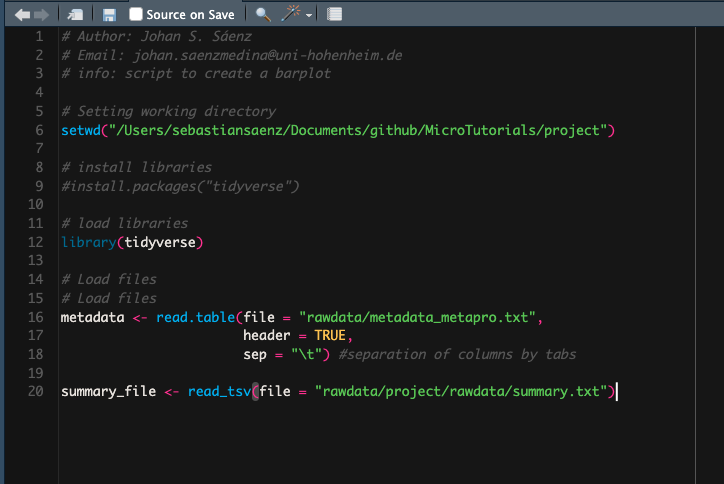
\includegraphics{script.png}

}

\end{figure}



\end{document}
